\documentclass[preprint,12pt]{elsarticle}
\usepackage{mathrsfs}
\usepackage{fancyhdr}
%\pagestyle{fancy}
\usepackage{verbatim}
\usepackage{graphicx}
\usepackage{graphics,color}
%\usepackage{bbding}
\usepackage{booktabs}
\usepackage{multirow}
\usepackage{tabularx}
\usepackage{amsmath,amssymb,amsthm}
%%The vector representation
\renewcommand{\vec}[1]{\boldsymbol{#1}}
%% General Constants e,i,pi and differetial operator
\newcommand{\me}{\mathrm{e}}
\newcommand{\mi}{\mathrm{i}}
\newcommand{\dif}{\mathrm{d}}
\newtheorem{hypothesis}{Hypothesis}

\begin{document}
\begin{frontmatter}
\title{Dynamics of a billiard-ball's collision with wall}
\author[nudt]{Dingwen Wang\corref{cor1}}
\ead{wangdingwen0618@gmail.com}
\author[nudt]{Puyun Gao}

\cortext[cor1]{Corresponding author, Tel:+86 15116442661}
\address[nudt]{College of Aerospace Science and Engineering, National University of Defense Technology, Changsha 410072, PR China}

\begin{abstract}
We consider a nonholonomic system with collisions and find that the instantaneous constraints conventionally regarded as nonholonomic are actually integrable. Besides, we take account of frictional impulse and propose a two-step impact model to describe the collision process. A billiard-ball jumps off the horizontal floor when it impacts with the vertical wall. Then the ball will fall back into the floor due to gravity. The formulations to relate the pre- and post-impact velocities are given. An example is given to show the discrepancy between the results of the conventional model and that of ours.
\end{abstract}
\begin{keyword}
  Nonholonomic system \sep Collision\sep Billiard-ball\sep Pure rolling motion
\end{keyword}
\end{frontmatter}

\graphicspath{{Figures/}}

\section{Introduction}\label{sec:intro}
In this article, we study the dynamics of a billiard ball which rolls without sliding on a rough horizontal plane collides with the vertical wall.
This is a typical nonholonomic system\cite{Neimark,Garwin,Gutkin,Treschev}.

Broomhead and Gutkin propose a model of a gas of rough hard balls which interact with each other and with the container walls through collision. They define the collisions as inelastic collisions which suggest the impulsive friction without slipping at the contact point conserves the total energy of the system. They restrict their model to 2 dimensions, so the balls are, in fact, discs on the smooth plane\cite{Gutkin}.
Dom\'emech uses a `discontinuous' model to describe billiard-ball collisions. He derives a series of formulations to relate the collision states with the impact angle and the coefficients of restitution and friction\cite{Domenech}.
Treschev and Zubelevich study the similar motion in the Lagrangian frame. Their treatment of this problem are rather mathematic\cite{Treschev}.

%Extra constraints are applied instantaneously to the system when collision occurs.
%Frictional impulse must be accounted for throughout the collision.

Generally, the collision is treated as instantaneous and there is a discontinuous change in the velocities of the ball.
%The ball often exhibits unexpected behaviors when it collides with each other or with a wall \cite{Garwin,Wallace}.
Conservation of kinetic energy and no sliding at the contact point are always assumed.
In fact, when the ball hits the wall, it will jump off the horizontal surface.
This effect is conventionally ignored by the authors for mathematical simplicity.
But it seems contradictory that one requires kinetic energy conserved while takes account of friction.
Here we treat the problem in a different manner which recognizes the role of friction.

Firstly, we study the collision using conventional assumptions. We find that the constraints usually considered as nonholonomic are essentially integrable. The formulations which describe the relation of velocities between the pre- and post-impact are given.
Next we establish a more realistic model which characterizes the collision as impacts of two-step. The model takes full account of the frictional impulse and the ball jumps off the floor after the first impact. We also find the total kinetic energy is not conserved even if the coefficient of restitution $e=1$, which makes some surprise. Finally, an example is given to show the discrepancy between the results of the conventional model and that of ours.

\section{Collision within the horizontal floor}\label{sec:collision}
Let's consider a billiard-ball rolls on a rough horizontal plane without sliding.
The homogeneous ball is set to be radius $a$ and mass $m$, so its center of mass coincides with its geometric center $C$.
The moment of inertia relative to any axis passing through the center $C$ is equal to $I$, which is $\frac{2}{5}m a^2$.

Supposing the rough vertical wall with which the ball collides be the $yOz$ plane, we establish a coordinate frame as Figure \ref{figure:coordinate}.
\begin{figure}[!hbt]
  \centering
  % Requires \usepackage{graphicx}
  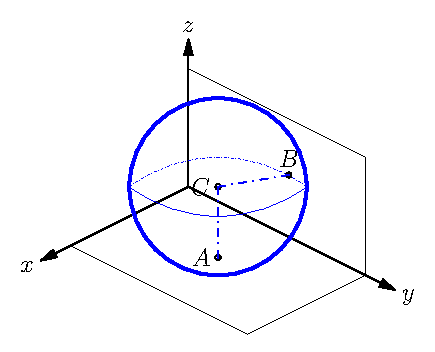
\includegraphics[scale=1]{myfirst.eps}\\
  \caption{Billiard-Ball collides with the wall}\label{figure:coordinate}
\end{figure}

The angular velocity $\vec{\omega}$ of the billiard-ball is expressed in terms of Eulerian angles $\theta, \varphi, \psi$:
\begin{equation}\label{eq:angular_velocity}
  \left\{\begin{array}{rcl}
  \omega_x&=&\dot{\theta}\cos \psi+\dot{\varphi}\sin \theta \sin \psi\\
  \omega_y&=&\dot{\theta}\sin \psi-\dot{\varphi}\sin \theta \cos \psi\\
  \omega_z&=&\dot{\varphi}\cos \theta+\dot \psi
  \end{array}\right.
\end{equation}
The constraints of no-sliding before collision are:
\begin{equation}\label{eq:Constraints_Ball_NoSliding}
 \left\{\begin{array}{rcl}
 \dot{x} &= &a (\dot{\theta} \sin\psi -\dot{\varphi}\sin\theta \cos\psi)\\
 \dot{y} &=& -a(\dot{\theta} \cos\psi +\dot{\varphi}\sin\theta \sin\psi)\\
 \dot{z} &=& 0
\end{array}\right.
\end{equation}
the first two equations are nonholonomic constraints.

By virtue of the constraints, the kinetic energy of the ball before collision is:
 \begin{equation}\label{eq:KineticEnergy_Ball_RoughPlain}
  T=\frac{1}{2}(m a^2+I)\dot{\theta}^2+\frac{1}{2}(m a^2\mathrm{sin}^2\theta+I)\dot{\varphi}^2+\frac{1}{2}I(\dot{\psi}^2+2\dot{\varphi}\dot{\psi}\cos\theta)
 \end{equation}

When the ball hits the wall at point $B$ which is the contact point of the ball and the wall, the additional constraints are instantaneously imposed on the system:
\begin{equation}
  \vec {V_{_B}}=\vec {V_{_C}}+\vec{\omega} \times \overline{CB}=\vec{0}
\end{equation}
Reducing them in terms of Eulerian angles, the constraints become to:
\begin{equation}
 \left\{\begin{array}{rcl}
 \dot \theta \sin \psi  - \dot \varphi \sin \theta \cos \psi & = &0\\
 \dot \theta \cos \psi  + \dot \varphi (\sin \theta \sin \psi  +\cos \theta ) +\dot \psi & = &0
 \end{array}\right.
\end{equation}
Choosing $\dot{\varphi}$ as independent velocity, we obtain from these equations
\begin{equation}\label{eq:Constraints_Ball_Wall}
 \left\{\begin{array}{rcl}
 \dot \psi & =&- \dot \varphi \left(\dfrac{\sin \theta }{\sin \psi } + \cos \theta \right)\\
 \dot \theta & = &\dot \varphi \sin \theta \cot \psi
 \end{array}\right.
\end{equation}
The two constraints are conventionally considered as nonholonomic constraints\cite{Neimark}, but in fact they are \textbf{integrable}.

Dividing the first equation by the second equation of \eqref{eq:Constraints_Ball_Wall}, we obtain:
\begin{equation}
  \dfrac{\dif\psi}{\dif\theta}=-\dfrac{\dfrac{\sin\theta}{\sin\psi}+\cos\theta}{\sin\theta \cot\psi}=-\dfrac{1+\cot\theta \sin\psi}{\cos \psi}
\end{equation}
This is a differential equation about $\psi$ in terms of $\theta$.
We can solve this equation without difficulty:
\begin{equation}
  \sin \psi =\frac{\cos \theta+c}{\sin \theta}
\end{equation}
$c$ is a constant. Assuming at the moment of collision $\varphi=\psi=0, \theta=\pi/2 $, the angular velocity becomes to $\vec{\omega}=(\dot{\theta},-\dot{\varphi},\dot{\psi})$. Then it follows that $c=0$, thus at the moment of collision the relation between $\psi$ and $\theta$ is:

 \begin{equation}\label{eq:Integration_First}
   \sin \psi=\frac{\cos \theta}{\sin \theta}=\cot \theta
 \end{equation}

We can also obtain the relation between $\varphi$ and $\theta$.
By virtue of the second equation of \eqref{eq:Constraints_Ball_Wall}, we have:

\begin{equation}
  \frac{\dif\varphi}{\dif\theta}=\frac{1}{\sin\theta \cot\psi(\theta)}
\end{equation}
as we have already known the relation between $\psi$ and $\theta$, this is also a differential equation about $\varphi$ in terms of $\theta$.
\[
\dif\varphi=\frac{\cos \theta \dif\theta}{\sin\theta \sqrt{2\sin^2\theta-1}}=\frac{ \dif\sin \theta}{\sin\theta \sqrt{2\sin^2\theta-1}}\quad(2\sin^2\theta-1>0)
\]
The final result is:
 \begin{equation}\label{eq:Integration_Second}
   \tan(\varphi-d)+\frac{1}{\sqrt{2\sin^2\theta-1}}=0\quad(2\sin^2\theta-1>0)
 \end{equation}
again, $d$ is a constant which need to be determined by initial conditions. Since we assume at the moment of collision $\varphi=\psi=0, \theta=\pi /2$, then $d$ is equal to $\pi/4$. We can also know that the assumption has satisfied the constraint $2\sin^2\theta-1>0$.

At last the constraints \eqref{eq:Constraints_Ball_Wall} are integrated to \eqref{eq:Integration_First} and \eqref{eq:Integration_Second}.

The conventional method to derive the equations of impulsive motion about nonholonomic systems is based on the d'Alembert-Lagrange principle with the so-called Chetaev conditions imposed on the virtual displacements. During the process of impact, the variations of the coordinates are restricted by the additional relations from \eqref{eq:Constraints_Ball_Wall}
\begin{equation}\label{eq:Chetaev_Condition}
 \left\{\begin{array}{rcl}
 \delta \psi  &=&- \delta \varphi \left(\dfrac{{\sin \theta }}{{\sin \psi }} + \cos \theta \right)\\
 \delta \theta & = &\delta \varphi \sin \theta \cot \psi
 \end{array}\right.
\end{equation}
But the validity of Chetaev conditions is controversial. Some scientist don't support Chetaev condition\cite{Guo}.
Since we have integrated the constraints \eqref{eq:Constraints_Ball_Wall}, the relations \eqref{eq:Chetaev_Condition} are still valid here. But they are no longer Chetaev conditions as in the conventional method, now they must be seen as the natural variations of two equations of holonomic constraints \eqref{eq:Integration_First} and \eqref{eq:Integration_Second}.

According to the equations of the impulsive motion given in the book\cite{Neimark}, we obtain
\begin{equation}
  \left(\frac{\partial \tilde{T}}{\partial \dot{\varphi}}\right)_1= \left(\frac{\partial \tilde{T}}{\partial \dot{\varphi}}\right)_0
\end{equation}
where the subscript $1$ refers to the post-impact state and the subscript $0$ to the pre-impact state. We denote by $\tilde{T}$ the kinetic energy $T$ which is a function of only $\dot{\varphi}$ and depends on $\dot{\varphi}$ not only explicitly but also implicitly through $\dot{\psi}$ and $\dot{\theta}$ by virtue of the relations \eqref{eq:Constraints_Ball_Wall}.
We differentiate \eqref{eq:KineticEnergy_Ball_RoughPlain}, taking $\dot{\varphi}$ as the independent velocity:
\begin{equation}
\begin{array}{rcl}
  \dfrac{\partial \tilde{T}}{\partial \dot{\varphi}}&=&\dfrac{\partial {T}}{\partial \dot{\varphi}}-\dfrac{\partial {T}}{\partial \dot{\psi}}\left(\dfrac{\sin \theta }{\sin \psi } + \cos \theta \right)+\dfrac{\partial {T}}{\partial \dot{\theta}}\sin \theta \cot \psi\\
  &= &\left(m a^2+I\right)\sin \theta \cot \psi \dot{\theta}-I\dfrac{\sin\theta}{\sin \psi}\dot{\psi} \\[12pt]
  & &{}+\left(m a^2 \sin^2 \theta+I \sin^2 \theta-I\dfrac{\sin \theta \cos \theta}{\sin \psi}\right)\dot{\varphi}
\end{array}
\end{equation}
Finally, the equations of the impulsive motion reduce to a single relation between the pre-impact and post-impact velocities:
\begin{equation}
\begin{array}{lrl}\label{eq:Impulsive_Motion}
  \left(m a^2+I\right)\cos\psi \Delta\dot{\theta}-I\Delta\dot{\psi}& &\\[12pt]
  +\left(ma^2\sin\theta \sin\psi+I\sin\theta \sin\psi-I\cos\theta\right)\Delta\dot{\varphi}&=&0
\end{array}
\end{equation}
where $\Delta\dot{\theta}=\dot{\theta}_1-\dot{\theta}_0,\Delta\dot{\varphi}=\dot{\varphi}_1-\dot{\varphi}_0,\Delta\dot{\psi}=\dot{\psi}_1-\dot{\psi}_0$.
As we have assumed that $\varphi=\psi=0, \theta=\pi/2$, the final form of equation \eqref{eq:Impulsive_Motion} is
\begin{equation}\label{eq:Velocity_Relation0}
   \left(m a^2+I\right)\left(\dot{\theta}_1-\dot{\theta}_0\right)-I\left(\dot{\psi}_1-\dot{\psi}_0\right)=0
\end{equation}
Since $\vec{\omega}=(\omega_x,\omega_y,\omega_z)=(\dot{\theta},-\dot{\varphi},\dot{\psi})$, equation \eqref{eq:Velocity_Relation0} becomes to
 \begin{equation}\label{eq:Velocity_Relation}
   \left(ma^2+I\right)\left(\omega_{x1}-\omega_{x0}\right)-I\left(\omega_{z1}-\omega_{z0}\right)=0
 \end{equation}

Obviously, the post-impact state cannot be determined by only equation \eqref{eq:Velocity_Relation}.
In order to obtain a further two equations, we make three hypothesis.
\begin{hypothesis}
  The ball remains rolling without sliding on the floor after impact.
\end{hypothesis}
\begin{hypothesis}
  The normal component of velocity is reversed by the impact.
\end{hypothesis}
\begin{hypothesis}
  The energy is conserved during the impact.
\end{hypothesis}

The first hypothesis means that the post-impact state is also characterized by three quantities $\dot{x}, \dot{y}$, and $\omega_z$.
We have
\begin{equation}
  \dot{x_i}= a\omega_{yi} ,\quad \dot{y_i} =- a\omega_{xi} ,\quad\dot{z_i} = 0\qquad (i=0,1)
\end{equation}

The second hypothesis suggests that the normal component of the velocity satisfies Newton's kinematic relation:
\begin{equation}\label{eq:Newton_Relation}
  \dot{x}_1=-e\dot{x}_0
\end{equation}
$e$ is the coefficient of restitution of the wall.

The kinetic energy of the ball is
\begin{equation}
  T_i=\frac{1}{2}m\left(\dot{x_i}^2+\dot{y_i}^2\right)+\frac{1}{2}I\left(\omega_{xi}^2+\omega_{yi}^2+\omega_{zi}^2\right),\qquad(i=0,1)
\end{equation}
For the energy is conserved, $e$ must be $1$, which implies :
\begin{equation}\label{eq:Energy_Conserved}
  T_0=T_1
\end{equation}

By virtue of \eqref{eq:Newton_Relation} and \eqref{eq:Energy_Conserved}, the following equations hold:
\begin{equation}\label{eq:State_Relation}
  \begin{split}
    \dot{x}_1&=-\dot{x}_0 \\
    \dot{y}_1&=\frac{m a^2}{2\left(I+m a^2/2\right)}\dot{y}_0+\frac{I a}{I+m a^2/2}\omega_{z0}\\
    \omega_{z1}&=\frac{I+m a^2}{\left(I+m a^2/2\right)a}\dot{y}_0-\frac{m a^2}{2\left(I+m a^2/2\right)}\omega_{z0}
  \end{split}
\end{equation}
The result here coincides with that of \cite{Treschev}.

\section{Collisions of Two--Step}\label{sec:collision_two_step}
\subsection{Discussion}
Now let's examine the impact process in more details.
For simplicity, we assume $\vec{V_{_C}}=(\dot{x}_0,\dot{y}_0,0)$ is the pre-impact velocity of the center of the ball. The ball is rolling without sliding and vertical spin on horizontal floor, which means
\begin{equation}
  \dot{x}_0-a\omega_{y0}=0,\quad \dot{y}_0+a \omega_{x0}=0,\quad\omega_{z0}=0
\end{equation}
The pre-impact velocity of the contact point $B$ is
\begin{equation}
  \vec{V_{_{B0}}}=\vec{V_{_C}}+\vec{\omega} \times \overline{CB}=(\dot{x}_0,\dot{y}_0,\dot{x}_0)
\end{equation}
According to equation \eqref{eq:State_Relation}, the post-impact velocity of Point $B$ is
\begin{equation}
  \vec{V_{_{B1}}}=(\dot{x}_{B1},\dot{y}_{B1},\dot{z}_{B1})=(-\dot{x}_0,-\dot{y}_0,-\dot{x}_0)
\end{equation}

Then the velocity of point $B$ experiences three states. $\vec{V_{_{B}}}=\vec{V_{_{B0}}}$ is the pre-impact velocity, while the post-impact velocity is $\vec{V_{_{B}}}=\vec{V_{_{B1}}}$. During the impact process(the interval is trivial, so it is can be seen as instantaneous), $\vec{V_{_{B}}}=\vec{0}$(section \ref{sec:collision}). The relation between the post-impact velocity and the pre-impact one is

\begin{equation}
  \vec{V_{_{B1}}}=-\vec{V_{_{B0}}}
\end{equation}

Of course this is the natural implication of the three hypothesis, but it is not reliable in physics.
Suppose the ball rolls without sliding because of Coulomb forces of friction.
Though the force doesn't produce work when the ball rolls on the floor, we must take it when the impact occurs.
The impulsive reaction of the wall has two components: the normal component is impulsive of restitution, while the tangential one is impulsive of friction.
The normal velocity will reverse($\dot{x}_{_1}=-\dot{x}_{_0}$) when we assume the coefficient of restitution $e=1$.
%The ball changes its velocity because of the reaction of the wall during impact.
But the force of friction can only deter the relative motion at the contact point $B$. It is unreasonable to say $\dot{y}_{_{B1}}=-\dot{y}_{_0},\dot{z}_{_{B1}}=-\dot{x}_{_0}$, which implies the forces of friction accelerate the ball in direction $Oy$ (from $\dot{y}_{_0}$ decelerates to $0$, and finally accelerates to $\dot{y}_{_{B1}}$) and $Oz$ (from $\dot{x}_{_0}$ decelerates to $0$, and finally accelerates to $\dot{z}_{_{B1}}$) at point $B$. This is contradictory to the sense of physics.

\subsection{The first impact}
Here we deduce a more realistic formulation to describe the impact process which considers the forces of friction.

\begin{figure}
  \centering
  % Requires \usepackage{graphicx}
  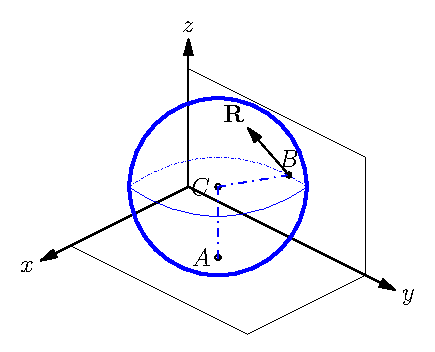
\includegraphics[scale=1]{mysecond.eps}\\
  \caption{Collision considering friction}\label{figure:collision}
\end{figure}


We assume that the impulsive forces of friction, as in the case of finite forces, will not exceed the $\mu$-fold value of the normal pressure, where $\mu$ is the coefficient of dry friction.
We must keep in mind that when the ball hits the wall, the impulse of reaction of the wall at point $B$ always has a positive vertical component.
It implies the ball is lifted during the impact and the forces of friction of the floor have no influence on the kinematics of the ball\cite{Neimark}.

We assume $\vec{V_{_C}}=(\dot{x}_0,\dot{y}_0,0)$ is the pre-impact velocity of the center of the ball($\dot{x}_0<0$), $\vec{\omega}=(\omega_{x0},\omega_{y0},\omega_{z0})$ is the angular velocity.
Point $A$ is the contact point of the ball and the floor.
By virtue of the condition of rolling without sliding:
\begin{equation}
  \dot{x}_0-a\omega_{y0}=0,\quad \dot{y}_0+a \omega_{x0}=0
\end{equation}
This means the pre-impact state can be determined by three parameters $\dot{x}_0,\dot{y}_0$, and the vertical spin $\omega_{z0}$.
$\vec{R}=(R_x,R_y,R_z)$ is the impulse of the wall at point $B$ (see Figure \ref{figure:collision}).

The equations of the impulse motion are
\begin{equation}
\left\{\begin{array}{rcl}
    m(\dot{x}_1-\dot{x}_0) &= & R_x \\
     m(\dot{y}_1-\dot{y}_0)& = & R_y\\
      m \dot{z_1} & = & R_z\\
    I(\omega_{x1}-\omega_{x0}) & = & 0\\
    I(\omega_{y1}-\omega_{y0}) & = & a R_z\\
    I(\omega_{z1}-\omega_{z0}) & = &-a R_y
\end{array}\right.
\end{equation}
Here we have only six equations for nine unknowns, so we need three more equations which depend on the impact conditions.
We assume that the normal component of the velocity satisfies Newton's kinematic relation \eqref{eq:Newton_Relation}.
When considering the tangential components of the velocity of the ball at point $B$, we assume $\vec{R}$ lies within the friction cone
\begin{equation}
  \sqrt{R_y^2+R_z^2}<\mu R_x
\end{equation}
Besides, point $B$ of the ball is not displaced tangentially during the impact, then we have:
\begin{equation}
  \dot{y}_1-a\omega_{z1}=0,\qquad \dot{z_1}+a \omega_{y1}=0
\end{equation}

Finally, we have nine equations for nine unknowns. Solving the equations, we get
\begin{equation}\label{eq:Result_After_First_Impact}
    \left\{\begin{array}{rclrclrcl}
      \dot{x}_1&=&-e\dot{x}_0,& \dot{y}_1&=&\frac{a\left( I \omega_{z0}+m a \dot{y}_0\right)}{ma^2+I},&\dot{z_1}&=&\frac{-I \dot{x}_0}{m a^2+I}\\[10pt]
    \omega_{x1}&=&-\frac{\dot{y}_0}{a},& \omega_{y1}&=&\frac{\dot{x}_0 I}{a\left(m a^2+I\right)},& \omega_{z1}&=&\frac{I \omega_{z0}+m a \dot{y}_0}{m a^2+I}\\[10pt]
    R_x&=&-m\dot{x}_0 \left(1+e\right),& R_y&=&\frac{m I\left(a\omega_{z0}-\dot{y}_0\right)}{m a^2+I},&R_z&=&-\frac{m \dot{x}_0 I}{m a^2+I}
    \end{array}\right.
\end{equation}
In this case, the velocity of point $B$ after impact $\vec{V_{_{B1}}}=(0,0,0)$ which is reasonable in the sense of physics.

It is noticeable that the kinetic energy here is not conserved.
For $e=1,\omega_{z0}=0$, we can get the kinetic energy before and after impact:
\begin{equation}
T_0=\frac{1}{2}m\dot{x}_0^2+\frac{1}{2}m\dot{y}_0^2+\frac{1}{2}I\frac{\dot{y}_0^2}{a^2}+\frac{1}{2}I\frac{\dot{x}_0^2}{a^2}
\end{equation}
\begin{equation}
T_1=\frac{1}{2}m \dot{x}_0^2+\frac{1}{2}\frac{m^2a^2\dot{y}_0^2}{I+ma^2}+\frac{1}{2}I\frac{\dot{y}_0^2}{a^2}+\frac{1}{2}\frac{I^2 \dot{x}_0^2}{a^2\left(I+ma^2\right)}
\end{equation}
It is clear that $T_1<T_0$.

\subsection{The second impact}
From equations \eqref{eq:Result_After_First_Impact}, we can see that the ball will leave the floor for $\dot{z}_1>0$( for  $\dot{x}_0<0$). Because of gravity the ball hits back to the floor with the velocity $(\dot{x}_1,\dot{y}_1,-\dot{z}_1)$, and the angular velocity remains.
Here we deduce the formulations which describe this impact process.
We describe the problem in this manner: a homogeneous ball of radius $a$ moves in an arbitrary state in space. At the instant of time $t_0$ it hits the floor.
By virtue of Eulerian angles, the kinetic energy of the ball is
\begin{equation}
  T=\frac{1}{2}m\left(\dot{x}^2+\dot{y}^2+\dot{z}^2\right)+\frac{1}{2}I\left(\dot{\theta}^2+\dot{\varphi}^2+\dot{\psi}^2+2\dot{\varphi}\dot{\psi}\cos \theta\right)
\end{equation}
When the ball hits the floor, the constraints \eqref{eq:Constraints_Ball_NoSliding} are imposed instantaneously. Here we have three independent general velocities: $\dot{\theta},\dot{\varphi}$ and $\dot{\psi}$:

\begin{equation}
\left\{\begin{array}{rcl}

    \frac{\partial \tilde{T}}{\partial \dot{\theta}} & = &\frac{\partial T}{\partial \dot{\theta}}+\frac{\partial T}{\partial \dot{x}}\frac{\partial \dot{x}}{\partial \dot{\theta}} +\frac{\partial T}{\partial \dot{y}}\frac{\partial \dot{y}}{\partial \dot{\theta}}\\
    &=&I\dot{\theta}+ma\sin\psi \dot{x}-ma\cos\psi \dot{y}\\[12pt]
    \frac{\partial \tilde{T}}{\partial \dot{\varphi}} & =&I\left(\dot{\varphi}+\cos\theta \dot{\psi}\right)-ma\sin\theta \cos\psi \dot{x}-ma\sin\theta\sin\psi \dot{y}\\[12pt]
    \frac{\partial \tilde{T}}{\partial \dot{\psi}} &=& I\left(\dot{\psi}+\cos\theta \dot{\varphi}\right)
  \end{array}\right.
\end{equation}
As in section \ref{sec:collision}, we can obtain the equations of the impulsive motion
\begin{equation}\label{eq:Impulsive_Motion_2}
  \left(\frac{\partial \tilde{T}}{\partial \dot{\theta}}\right)_1=\left(\frac{\partial \tilde{T}}{\partial \dot{\theta}}\right)_2,\left(\frac{\partial \tilde{T}}{\partial \dot{\varphi}}\right)_1=\left(\frac{\partial \tilde{T}}{\partial \dot{\varphi}}\right)_2,\left(\frac{\partial \tilde{T}}{\partial \dot{\psi}}\right)_1=\left(\frac{\partial \tilde{T}}{\partial \dot{\psi}}\right)_2
\end{equation}
Subscript $2$ refer to the post-impact state in this step.
We assume after the impact, constraints \eqref{eq:Constraints_Ball_NoSliding} hold. This means the coefficient of the restitution of the floor $e=0$ and the ball rolls without sliding after the impact.

Also assuming at the moment of collision $\varphi=\psi=0, \theta=\pi/2$ , we have the angular velocity $\vec{\omega}=(\omega_x,\omega_y,\omega_z)=(\dot{\theta},-\dot{\varphi},\dot{\psi})$. Equations \eqref{eq:Impulsive_Motion_2} become to
\begin{equation}
\left\{\begin{array}{rcl}
    I\omega_{_{x2}}-ma\dot{y_2}&=&I\omega_{_{x1}}-ma\dot{y}_1\\
    I\omega_{_{y2}}+ma\dot{x_2}&=&I\omega_{_{y1}}+ma\dot{x}_1\\
    I\omega_{_{z2}}&=&I\omega_{_{z2}}
\end{array}\right.
\end{equation}
Constraints \eqref{eq:Constraints_Ball_NoSliding} become to
\begin{equation}
\left\{\begin{array}{rcl}
  \dot{x}_2&=&a\omega_{_{y2}}\\
  \dot{y}_2&=&-a\omega_{_{x2}}\\
  \dot{z}_2&=&0
  \end{array}\right.
\end{equation}
The final result is
\begin{equation}\label{eq:Result_After_Second_Impact}
\left\{\begin{array}{rcl}
    \dot{x}_2&=&\frac{a\left(I\omega_{_{y1}}+ma\dot{x}_1\right)}{I+ma^2} \\[6pt]
    \dot{y}_2&=&\frac{a\left(ma\dot{y}_1-I\omega_{_{x1}}\right)}{I+ma^2} \\[6pt]
    \dot{z}_2&=&0\\[6pt]
    \omega_{_{x2}}&=&\frac{I\omega_{_{x1}}-ma\dot{y}_1}{I+ma^2}\\[6pt]
    \omega_{_{y2}}&=&\frac{I\omega_{_{y1}}+ma\dot{x}_1}{I+ma^2}\\[6pt]
    \omega_{_{z2}}&=&\omega_{_{z1}}

  \end{array}\right.
\end{equation}

By \eqref{eq:Result_After_First_Impact} and \eqref{eq:Result_After_Second_Impact} we can know the relationship between the initial state of the ball and its final state after impacts of two-step.
\section{Example}
To illustrate and compare the models developed in the preceding sections, we present a simple example.

Consider a ball moves without sliding on the rough floor, its velocity is $(-u_0,v_0,0)$ and there is no vertical spin which means $\omega_{z1}=0$($u_0>0,v_0>0$). Assuming the coefficient of restitution of the wall $e_{wall}=1$ and that of the floor $e_{floor}=0$, the state of the ball after the first impact is:
\begin{equation}
\left\{\begin{array}{rcl}
    \dot{x}_1 & =&u_0 \\[6pt]
    \dot{y}_1 & =&\frac{ma^2}{I+ma^2}v_0=\frac{5}{7}v_0\\[6pt]
    \dot{z}_1 & =&\frac{Iu_0}{I+ma^2}=\frac{2}{7}u_0\\[6pt]
    \omega_{_{x1}} & =&-\frac{v_0}{a}\\[6pt]
    \omega_{_{y1}} & =&-\frac{u_0 I}{a\left(m a^2+I\right)}=-\frac{2}{7}\frac{u_0}{a}\\[6pt]
    \omega_{_{z1}} &=&\frac{m a v_0}{m a^2+I}=\frac{5}{7}\frac{v_0}{a}\\[6pt]
    \end{array}\right.
\end{equation}
The state of the ball after the second impact is:
\begin{equation}\label{eq:example}
\left\{\begin{array}{rcl}
    \dot{x}_2 & =&\frac{31}{49}u_0 \\[6pt]
    \dot{y}_2 & =&\frac{39}{49}v_0 \\[6pt]
    \dot{z}_2 & =&0\\[6pt]
    \omega_{_{x2}} & =&-\frac{39}{49}\frac{v_0}{a}\\[6pt]
    \omega_{_{y2}} & =&\frac{25}{49}\frac{u_0}{a}\\[6pt]
    \omega_{_{z2}} &=&\frac{5}{7}\frac{v_0}{a}\\[6pt]
    \end{array}\right.
\end{equation}

\begin{figure}[!htb]
\centering
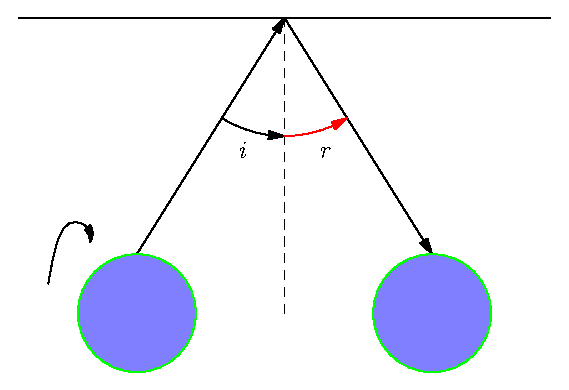
\includegraphics[scale=0.8]{billiardimpact}
\caption{Incidence and Reflection} \label{figure:incidence_reflection}
\end{figure}

Now we can obtain the relation between the incidence angle and the reflection angle by equation \eqref{eq:example}: $\tan\tau_{i}=\frac{v_0}{u_0}$ and $\tan\tau_{r}=\frac{39}{31}\frac{v_0}{u_0}$.
If $u_0=v_0$, the angle of incidence is $45^{\circ}$, then the final angle of reflection is $\arctan\frac{39}{31}\approx51.5^{\circ}$(see Figure \ref{figure:incidence_reflection}).
In contrast we use the method in section \ref{sec:collision}, the result is $\dot{x}_1=u_0, \dot{y}_1=\frac{5}{9}v_0, \omega_{z1}=\frac{14}{9}\frac{v_0}{a}$ and the angle of reflection will be $\arctan\frac{5}{9}\approx29.1^{\circ}$, which is much smaller than the previous one.

\section{Conclusion}

In this paper, we study the nonholonomic system with collision: a billiard-ball rolling without sliding impacts with the vertical wall. We find that the constraints instantaneously imposed to the system are actually integrable when impact occurs. So the conventional Chetaev conditions can be avoided in this problem.

We also establish a two--step collision model for this problem. The ball will leave the floor when it hits the vertical wall due to the frictional impulse. We take account of this effect which is conventionally ignored. The collision should be separated into two steps. The ball will fall back to the horizontal floor after its first impact with the vertical wall. The kinetic energy of the ball is not conserved in this process which is more realistic.

``Angle of incidence equals angle of reflection" is true only in a frictionless world\cite{Wallace}. In our model, the final reflection angle is greater than the incidence angle which is a contrast to the result of the conventional energy conserved model. To test which one is valid, we need play an actual billiard-ball game to observe the relation of angles.


\begin{thebibliography}{99}
\setlength{\parskip}{0pt}  %
\bibitem{Neimark} Neimark, Ju.I., Fufaev, N.A. Dynamics of Nonholonomic systems. Amer. Math. Sco. Rhode Island, 1972.
\bibitem{Garwin} Garwin, R. Kinematics of an Ultrelastic Rough Ball. Amer. Journ. of Physics 1969;37:88-92.
\bibitem{Gutkin} Broomhead, D.S., Gutkin, E. The dynamics of billiards with no-slip collisions. Physica D 1993;67:188-197.
\bibitem{Guo} Guo, Z.H. Rational solutions to a class of nonholonomic systems. Science in China (Series A) 1994;37:433-449.
\bibitem{Domenech} Dom\'enech, A. Non-smooth modelling of billiard- and superbilliard-ball collisions. International Journal of Mechanical Sciences 2008;50:752-763.
\bibitem{Treschev} Treschev, D., Zubelevich, O. On Collisions in Nonholonomic Systems. http://arxiv.org/abs/1206.1496v5

\bibitem{Wallace} Wallace, R.E., Schroeder, M.C. Analysis of billiard ball collisions in two dimensions. Amer. Journ. of Physics 1988;56:815-819.
\end{thebibliography}
\end{document}
